\documentclass[12pt]{article}
\usepackage{fontspec}
%\setromanfont{SimSun}
\setmainfont{Times New Roman}
\usepackage{amsmath, amssymb}
\usepackage{setspace}
\usepackage{textcomp}
\usepackage{fancyhdr}
\usepackage{lastpage}
\usepackage{indentfirst}
\usepackage{graphicx}
\usepackage{booktabs}
%\usepackage{txfonts}

\pagestyle{fancy}
\usepackage{lastpage}
\lhead{Team \# 0000}
\rhead{Page \thepage{} of  \pageref{LastPage}}
\cfoot{}		

\begin{document}

\begin{center}
\Large Methods of Detecting the Criminals Using Network Analysis
\end{center}

\begin{center}
\large Summary
\end{center}

	In this paper, we build the network model to analyse and detect the conspirators hidden in a network organization and find out their leader.
	
	For the first requirement, analyzing the EZ case, conspirators tend to have frequent communication and similar message communication with other conspirators. Based on graph theory, we introduce two concepts, Suspicion parameter and Crime centrality to quantity the suspicious degree of a person in the network. Then we use Topsis algorithm to prioritize the conspiracy scheme possibility of a person What’s more, we can find \textbf{Seeni} is the most potentially criminal leader in this case by analyzing the topics of conversations he has with the known conspirators and the suspicious message he has. 

	For the second requirement, when topic 1 are considered as suspicious question and Chris converts to be conspirator, we get a new ranking list and compare it to the ranking list before.

	For the third requirement, semantic network analysis is employed to enhance the sensitivity of our model. Thus, we can abstract key words from message flows to gather the information we need. After this, we get another ranking lists of the conspirator possibility. Comparing to the ranking list before, we come to several interesting conclusions. What’s more, the suspicious leader of this conspiracy crime remains unchanged.
 
	After that, we apply our model in other fields which differ from criminal network. Under different circumstances, we add other parameters to improve the accuracy. Using the graph theory, we state a general approach to identify, prioritize, and categorize similar nodes in a network. 

	Finally, the strengths and weaknesses of the model are discussed, and the future work is pointed out.

\vspace{5cm}

\tableofcontents

\vspace{8cm}

\section{Introduction}
\subsection{Background}
        
        In a information-based society, the development of data network is getting increasingly faster. As a result, the relations between people who  are involved into the social network become more complicated. In order to methodize the massive data in the network, the network analysis model comes into being. These models of connection between people describes mutual relations in the aspect of point set, entropy and macro-statistics, which largely simplify  the sophisticated social phenomenon and provides a  way to forecast the future development. Now the network analysis model has been widely applied to analyse social individuals’ connections, comprehend the social structure\cite{A1}\cite{A2} and investigate the communication system in large group of organization\cite{A3}\cite{A4}.    
	
	Among them, crime network receives particular attention in  determining the criminal organizations\cite{A5}. This paper mainly focuses on identifying criminal conspirators on the background of a conspiracy in a software company.We are going to find out the potential criminals with provided pieces of evidence.
	
\subsection{Our Work}

	Noticing that there are some problems in the data given, we deal with them as follows: 
\begin{itemize}
\item There five groups of people with the same name in the message traffic and Elsie is one of them. Since Elsie is a known conspirator, we make a decision that Elsie whose number is 7 is the conspirator knownand the other remains to be seen. 
\item There is a strange message that node 3 talked to himself in the message traffic. We avoid this invalid data.
\end{itemize}
	First,the possibility of a node being a conspirator performs not only in the his coonection of the whole company netwrok,but also in his connection with the known conspirators and suspicious message topics.In order to get a clear picture of the problem, we think that three factors should be taken into consideration to measure the possibility of a node being a conspirator:
\begin{itemize}
\item The person’s extensive degree in the network of company.
\item The times of communication with known conspirators.
\item The number of known suspicious message topics sent by himself and received by others.
\end{itemize}
	The measure of the possibility of a conspirator being a leader should contain the following factors:
\begin{itemize}
\item The possibility of the nodes he communicates directly being a conspirator.
\item The possibility of the nodes he communicates indirectly being a conspirator.
\end{itemize}

	On the basis of above discussion, to discover all the conspirators of a criminal gang ,to find its leader, and to promote it to be applied in other fields, we may boil down the tasks to the following five questions:
\begin{enumerate}
\item Adapting criminal analysis, we will give a priority list , determine the conspirators and find the leader of the criminal gang.
\item Adding the known information to the before model and analyze what changes happen in the before results,
\item Add semantic network analysis into the model to refine it.
\item Extending previous models and algorithms,State a general approach by which can identify, prioritize, and categorize similar nodes in a network in other actual fields to examine their adaptability ., 
\item Discuss the science and utility of the model built before
\end{enumerate}

\section{Assumptions} 
	We make these following assumptions about the criminal data in this paper.
\begin{itemize}
\item We assume that the resource of message traffic is reliable and all the information is true.
\item In order to simplify the model, we neglect the time factor in conversations.
\item According to the basic information we receive, we assume that only one single  criminal organization exists in the process of our model construction.
\end{itemize}

\section{Symbol Descriptions}

In this section, we use symbols  for constructing the model as follows.


\begin{table}[!htb]
\centering
\arrayrulewidth0.8pt
\begin{tabular}{c|c}
\toprule[2pt] 
\textbf{Symbol} & \textbf{Meaning} \\
\hline
$P_i$ & relevant vectors of node $i$ \\
$W(k)$ & the weight of topic $k$ \\
$send(i,j,k)$ & quantity the fact whether $i$ sends messages about topic $k$ to node $j$ \\
$A_{ij}$ & potential relation degree  with the conspirators \\
$B_{ij}$ & information similarity \\
$V_{ij}$ & the node $i$ receives or sends topic $j$ \\
$CE_i$ & the closeness of connection of the nodes \\
$CN_i$ & the closeness of connection of the edges \\
\hline
\end{tabular}
\end{table}
\begin{flushright}
P.s:Other symbol instructions will be given in the text
\end{flushright}



\section{Crime Detection}
	After researching several papers in relevance of crime network field, we draw some regular common conclusions on this special kind of network.
\begin{enumerate}
\item The diameter of crime network usually isn’t great. Thus, most networks enjoy a high density.
\item The level of information sharing is equal.
\item Most networks have radial center.
\end{enumerate}
	
	With Feature (1) and Feature (2) we can analyse the criminal potentiality in the crime network. Besides, Feature (2) can help us to identify the conspiracy leaders in the whole relations.
	Through these common features, we apply these into practical problems and establish the following models to tackle with the problem.
	Before modeling, to avoid ambiguity, we define the two concept here:
\begin{enumerate}
\item Suspicion parameter: we employ to measure the suspicious degree of one node.
\item Crime centrality: This parameter is used to quantity one node’s closeness to the criminal center.
\end{enumerate}


\subsection{Model One: Criminal Digging Algorithm Based on Connection Law}
	Connection law is a method to determine the high frequency of communication between two people under the circumstances of concentrative distribution of data. In this case, the investigators has formed the people and message network. Thus, we are able to carry on a series of deeper data mining.
	In order to find suspicious degree of each person in this company, according to graph theory, we define the nodes as people and the sides as the communication among these people. Thus, we establish network model which can reflect the relation among people in this company.In Figure \ref{F2} we take the suspicious talk among people into account as the relations in the network to get the connection relationship in the company.
         To evaluate the suspicious degree  of each person in the network model, we discuss its measuring method in the following section.

\begin{figure}[!htb]
\centering
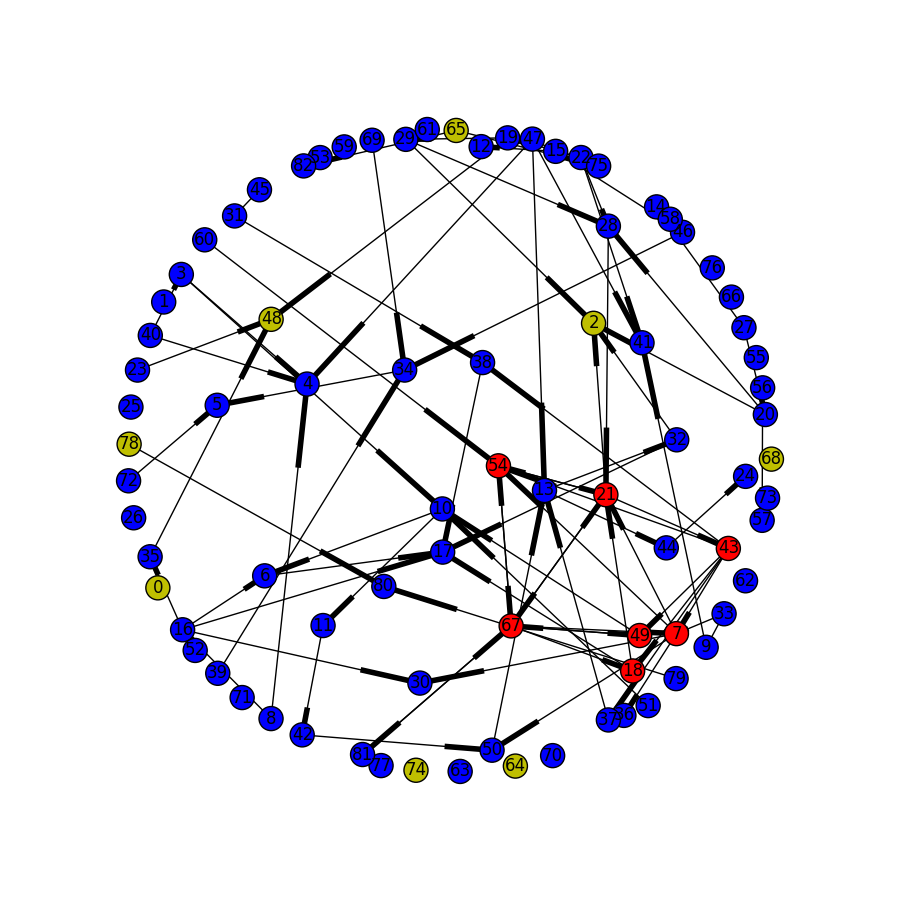
\includegraphics[width=6cm]{fig7_11_13_1.png}
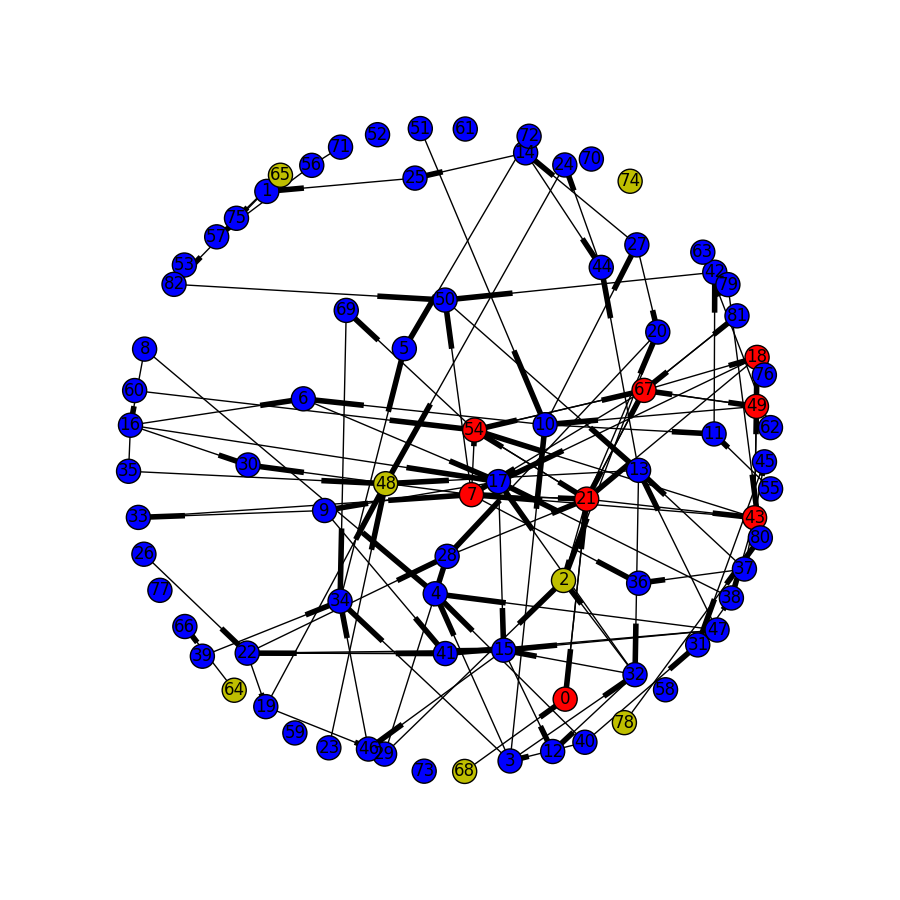
\includegraphics[width=6cm]{fig7_11_13_2.png}
\caption{\textbf{Before we move Chris(Left) and After we move Chris(Right)}}
\label{F2}
\end{figure}


\subsubsection{Suspicion Detection via the importance of node}
	In this model, we introduce the conception of potential relation degree with the conspirators as $A_{ij}$.Through the number of $A_{ij}$ nodes, we can build the connection path from node $i$ to node $j$.
	The proportion of indirect connection of nodes is the proportion of sides with same nodes and the joint nodes, which can be expressed as:
\begin{equation}
\centering
A_{ij} = \frac{P_i \bigcap P_j}{P_i \bigcup P_j}
\end{equation}
\begin{equation}
\centering
AA_i = \frac{1}{n}\sum_{j=1}^{n}A_{iS_j}
\end{equation}
	In this equation, $O$ is the row vector with each value being 1, $P_i$ represents relevant vectors of node i.  refers to the number of node which represents the people in the network.
	However, after reviewing the cases provided by our supervisor, we notice that the nodes which enjoy high level of connection with others in the network don’t directly mean that they are under high level of suspicion. Take Carol for example, although he has direct conversations with most people in the company, the relevant topics are not about the known suspicious topics. The single use of connection degree to measure the importance of node may indicate errors. Therefore, we can conclude that the potential connection with criminals can represents the direct connecting ability with its suspicious node, but it cannot perfectly reflect the criminal message he receives .As a result, we decide to use the information similarity to evaluate one person’s suspicious degree.
	
\subsubsection{Determining Suspicion Degree with Information Similarity}

	Here,we introduce several parameters to help us measure the suspicion degree.We use $W(k)$ to represent the weight of topic $k$.To help us quantity the value of connection, we use the function send(i,j,k), which is defined as follows: If node $i$ sends messages about topic $k$ to node $j$, then the value of send(i,j,k) is 1, or it is 0.
\begin{equation}
\centering
W(k) = \sum_{i=1}^n \sum_{j=1}^n send(i,j,k)
\end{equation}

	And, We employ the concept of $information similarity$ as  $B_{ij}$. It is defined as:
\begin{equation}
\centering
B_{ij} = \frac{(V_i \bigcap V_j) \times W^T}{(P_i \bigcup P_j) \times W^T}
\end{equation}
	$V_{ij}$ represents the node $i$ receives or sends topic $j$. So $V_i$ can express the relevant eigenvector of node $i$ concerning all the topics. In the same way as the calculation of $AA_i$, we can get the value of $BB_i$,which describes mean of the information similarity.

\subsubsection{Topsis Algorithm}
	Topsis algorithm see the parameters which may affect the results of the evaluation of $N$ indicators as the $N$ axis, constructing an $N-dimensional$ space, and then select the best value and the worst value of the index from all the objects to be evaluated. Then we use it to depict two points in N-dimensional space, which are respectively the best node and the worst node. Then we can calculate each the distance of objects to be evaluated to both worst and best points via the coordinates of the points, expressed as $D_{best}$ and $D_{bed}$.

	The smaller the value of result is, the better evaluation result one index has. In order to minimize the errors in analysis, we use the two index of suspicion parameter, $AA_i$ and $BB_i$, and employ the Topsis Algorithm to determine the final suspicion parameter $CC_i$.

	
\subsection{Model Two: Conspiracy Leader Model}
	As is expressed in the beginning of this part, the concept of criminal centrality is used here.
	Here, two parameters which respectively describes the closeness of connection of the nodes and the edges are introduced here as $CE_i$ and $CN_i$. In the network built on the conversations of suspicious topics, we choose the child network whose center is node i and calculate its value of $CE_i$ and $CN_i$.
\begin{equation}
\centering
CN_i = \frac{\sum CC_j}{\sum_{k=all} CC_k} , dis(i,j) \le 1
\end{equation}
	And the calculation method of  $CE_i$ is the same as $CN_i$.With these indices, we can get the value of the criminal centrality with Topsis Algorithm.

\section{Semantic Network Analysis}
	Because the leader provides us with the text evidence about the case,we introduce semantic network analysis to obtain and understand this message traffic. Based on the conversation we accumulate, we abstract the key words in each part. Then we sort out the simple semantic network with these key topics. The text connection of the people who have been identified are shown in Figure \ref{F1}.

%%%%%%%%%%%%%%%%%%%%%%%%%%%%%%%%%%%%%%%%%%%%%%
%图形排版样式4:两个图片并列,分别取名
%图形排版时名称一般都在下方
\begin{figure}
\begin{center}
\begin{minipage}[c]{0.5\textwidth}
\centering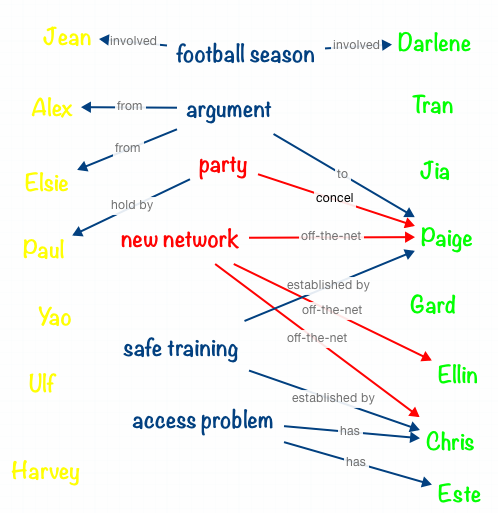
\includegraphics[width=6cm,height=6cm]{netwrok1.png}%就在前面括号中写图片名
\renewcommand{\figurename}{\textbf{Fig}}
\caption{L}
\label{F1}
\end{minipage}%
\begin{minipage}[c]{0.5\textwidth}
\centering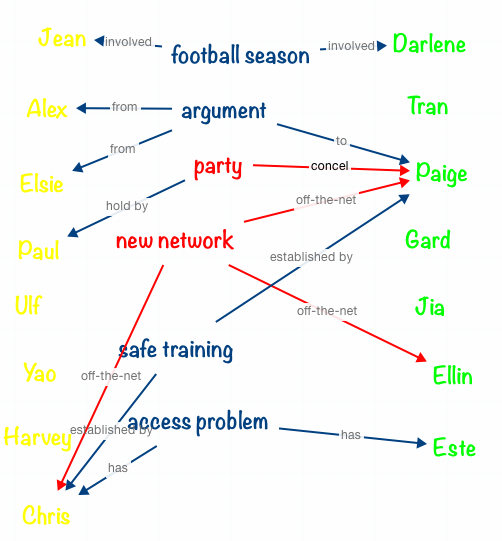
\includegraphics[width=6cm,height=6cm]{network2.png}%就在前面括号中写图片名
\renewcommand{\figurename}{\textbf{Fig}}
\caption{R}
\label{F3}
\end{minipage}
\end{center}
\end{figure}
%

	In Figure \ref{F1} and Figure the edges about suspicious plotting information are highlighted with red color. Then we can move these edges to simplify the figures. Then we can use the model in 4.1 and 4.2 to rank the probability of the conspiracy of people

\section{Conclusions}

\begin{table}[!htb]
\centering
\arrayrulewidth0.8pt
\begin{tabular}{c|c|c|c|c}
\toprule[2pt] 
\textbf{Rank} & \textbf{Name} & \textbf{Number} & \textbf{Suspicion Parameter} & \textbf{Crime Centrality} \\
\hline
1 & Seeni & 81 & 0.971127 & 0.285877 \\
2 & Priscilla & 36 & 0.489603 & 0.070006 \\
3 & Elsie & 37 & 0.470851 & 0.080407 \\
4 & Neal & 17 & 0.469860 & 0.105787 \\
5 & William & 50 & 0.455412 & 0.064059 \\
6 & Stephanie & 30 & 0.455224 & 0.054323 \\
7 & Dolores & 10 & 0.453054 & 0.142427 \\
8 & Beth & 38 & 0.449640 & 0.077608 \\
9 & Dwight & 28 & 0.303567 & 0.074443 \\
10 & Marion & 13 & 0.132587 & 0.078109 \\
\hline
\end{tabular}
\caption{\textbf{the top 10 in Requirement 1}}
\label{2_7_8}
\end{table}

\begin{table}[!htb]
\centering
\arrayrulewidth0.8pt
\begin{tabular}{c|c|c|c|c}
\toprule[2pt] 
\textbf{Rank} & \textbf{Name} & \textbf{Number} & \textbf{Suspicion Parameter} & \textbf{Crime Centrality} \\
\hline
1 & Seeni & 81 & 0.938551 & 0.243349 \\
2 & Crystal & 20 & 0.774827 & 0.075497 \\
3 & Dwight & 28 & 0.618407 & 0.087823 \\
4 & Han & 69 & 0.567552 & 0.044596 \\
5 & Priscilla & 36 & 0.556685 & 0.058212 \\
6 & Stephanie & 30 & 0.526444 & 0.046208 \\
7 & Neal & 17 & 0.518843 & 0.113929 \\
8 & William & 50 & 0.517807 & 0.062367 \\
9 & Dolores & 10 & 0.498024 & 0.133087 \\
10 & Elsie & 37 & 0.488753 & 0.070420 \\
11 & Lois & 45 & 0.479205 & 0.045231 \\
12 & Beth & 38 & 0.474695 & 0.067759 \\ 
13 & Malcolm & 9 & 0.207755 & 0.038849 \\
\hline
\end{tabular}
\caption{\textbf{the top 13 in Requirement 2 after moving Chris}}
\label{2_8_7}
\end{table}

From the Table \ref{2_7_8} and Table \ref{2_8_7}, we can conclude that:
\begin{enumerate}
\item People who have more connections with suspicious people rank higher in the table where we take the crime information into account.
\item The fact that the core people in the crime network remains the same can show us that the leader position can be roughly analysed by the conversation frequency.
\end{enumerate}

\section{Further Analysis}
\subsection{Strengths and Weaknesses}
\subsubsection{Strengths} 
\begin{itemize}
\item We take both the node position in the whole network and suspicious message it sends and receives into consideration for identifying and prioritizing conspirators. So, the solution of our model pursues high credibility, while reducing the misjudgment rate. 
\item The result of simulation shows that our model can be applied to other field, so it is extendable.
\item The result of our model match perfectly with the experience, which proves the reasonability of our model .
\end{itemize}

\subsubsection{Weaknesses}  
\begin{itemize}
\item Since there is no clear criteria for the classification, those conspirators who are slightly behind may be missed. 
\item We don‘t take the Criminal Psychology into consideration while to mix the detective’s judgement,what some people say may not true.
\item In actual situations,criminal gang may be more handsome and the hidden boss may be hidden deeply so that our model has possibility to loss them.
\end{itemize}

\subsection{Future work} 
\begin{enumerate}
\item Apply semantic network analysis to discover the potential linkage between the messages and scientifically classify them into different groups. 
\item Find a more reasonable criteria for the classification and consider the Criminal Psychology for dealing with more complex and specific cases.
\end{enumerate}

\section{Model Extension}
In our model , we use many network techniques to empower our model. And in common network analysis, we often use indexes about nodes and edges . What’s more ,in a specific network, there are always related information about nodes and edges . We both use the common and feature of network to build our model, with the goal that making the estimating result more accurate.While dealing with the problem of crime busting, we take some specific features such as suspicious topics and persons .It is the same with similar problems like assuming the infection ability of different cells.
Based on these conclusions above, we state a general approach, by which can identify, prioritize, and categorize similar nodes in a network as follows: 
\begin{itemize}
\item First, collect datas of various properties of nodes in the network and analyze them to estimate general characteristics of that network. 

\item Then, according to features of specified network, transform them into indexes about nodes and edges just like what we do in our model. 

\item Finally, combine both of them together into a weighted average. And that is a score mesures nodes with the given standard. With this score of result, we can identify, prioritize, and categorize similar nodes in that network.
\end{itemize} 


\begin{thebibliography}{99}
\bibitem{A1}
XU JJ, CHEN HC. CrimeNet Explorer: A Framework for Criminal Network Knowledge Discoveryp[J].ACM Transactions on Information Systems, 2005, 23(2).
\bibitem{A2}
BERKOWTTZ SD. An Introduction on Structural Analysis : The Net work Approach to Social Research[M].Butterworth, Toronto, 1982.
\bibitem{A3}
BREIGER RL. The analysis of social networks[A]. HARDY MA, BRYMAN A, eds. Handbook of Data Analysis. Sage Publications, London, UK, 2004.505 – 526.
\bibitem{A4}
GARTON L, HAYTHORNTHWATTE C, WELLMAN B. Studying online social networks[A] . JONES S, Ed. Doing Internet Research[C]. Sage Publications, London, UK, 1999.75 – 105.
\bibitem{A5}
CHANGJIE TANG, WEI LIU, FENLIAN WEN, SHAOJIE QIAO. Three explorations in social network analysis and organization information digging:find the structure and core of virtual organization and communication behaviors[J].Computer applications,2006-2020-04
\bibitem{A6}
CHEN DONG, CUNLE QIAN, JIANJUN MA.Crime network detection based on social network analysis[J].Mathermatical Model Construction and Applications,2012-0072-11
\end{thebibliography}

\end{document} 